
I projektet er der blevet arbejdet på fire studieområder i Danmark. De fire studieområder er Aabenraa, Gedser Havn, Hesnæs og Præstø.\\

Til udvælgningen af studieområderne blev i alt otte kommuner kontaktet. Dette inkluderer Aabenraa, Faaborg-Midtfyn, Guldborgsund, Haderslev, Stevns, Sønderborg og Vordingborg. Denne udpegning af potentielle lokaliteter skete på baggrund af en tabel fra \cite{damberg_vaerste_2023} over højeste målte vandstande i Danmark under oktober 2023 stormfloden. 
Ud af de otte kommuner blev tre kommuner (Aabenraa, Guldborgsund og Vordingborg) udvalgt til videre samarbejde på baggrund af tilgængeligt data. Guldborgsund kommune stillede data fra fire lokaliteter i kommunen til rådighed og der blev udvalgt de to kystbyer, Gedser Havn og Hesnæs, på baggrund af højere målt vandstand under stormflode i oktober 2023. \\

De fire udvalgte studieområder er lokaliseret langs sydkysten af Danmark. På figur \ref{Figur: Oversigtskort} er områdernes placering i Danmark visualiseret. Alle fire lokaliteter oplevede forhøjet vandstand under stormfloden den 20.-21. oktober 2023. 
\begin{figure}[H]
    \centering
    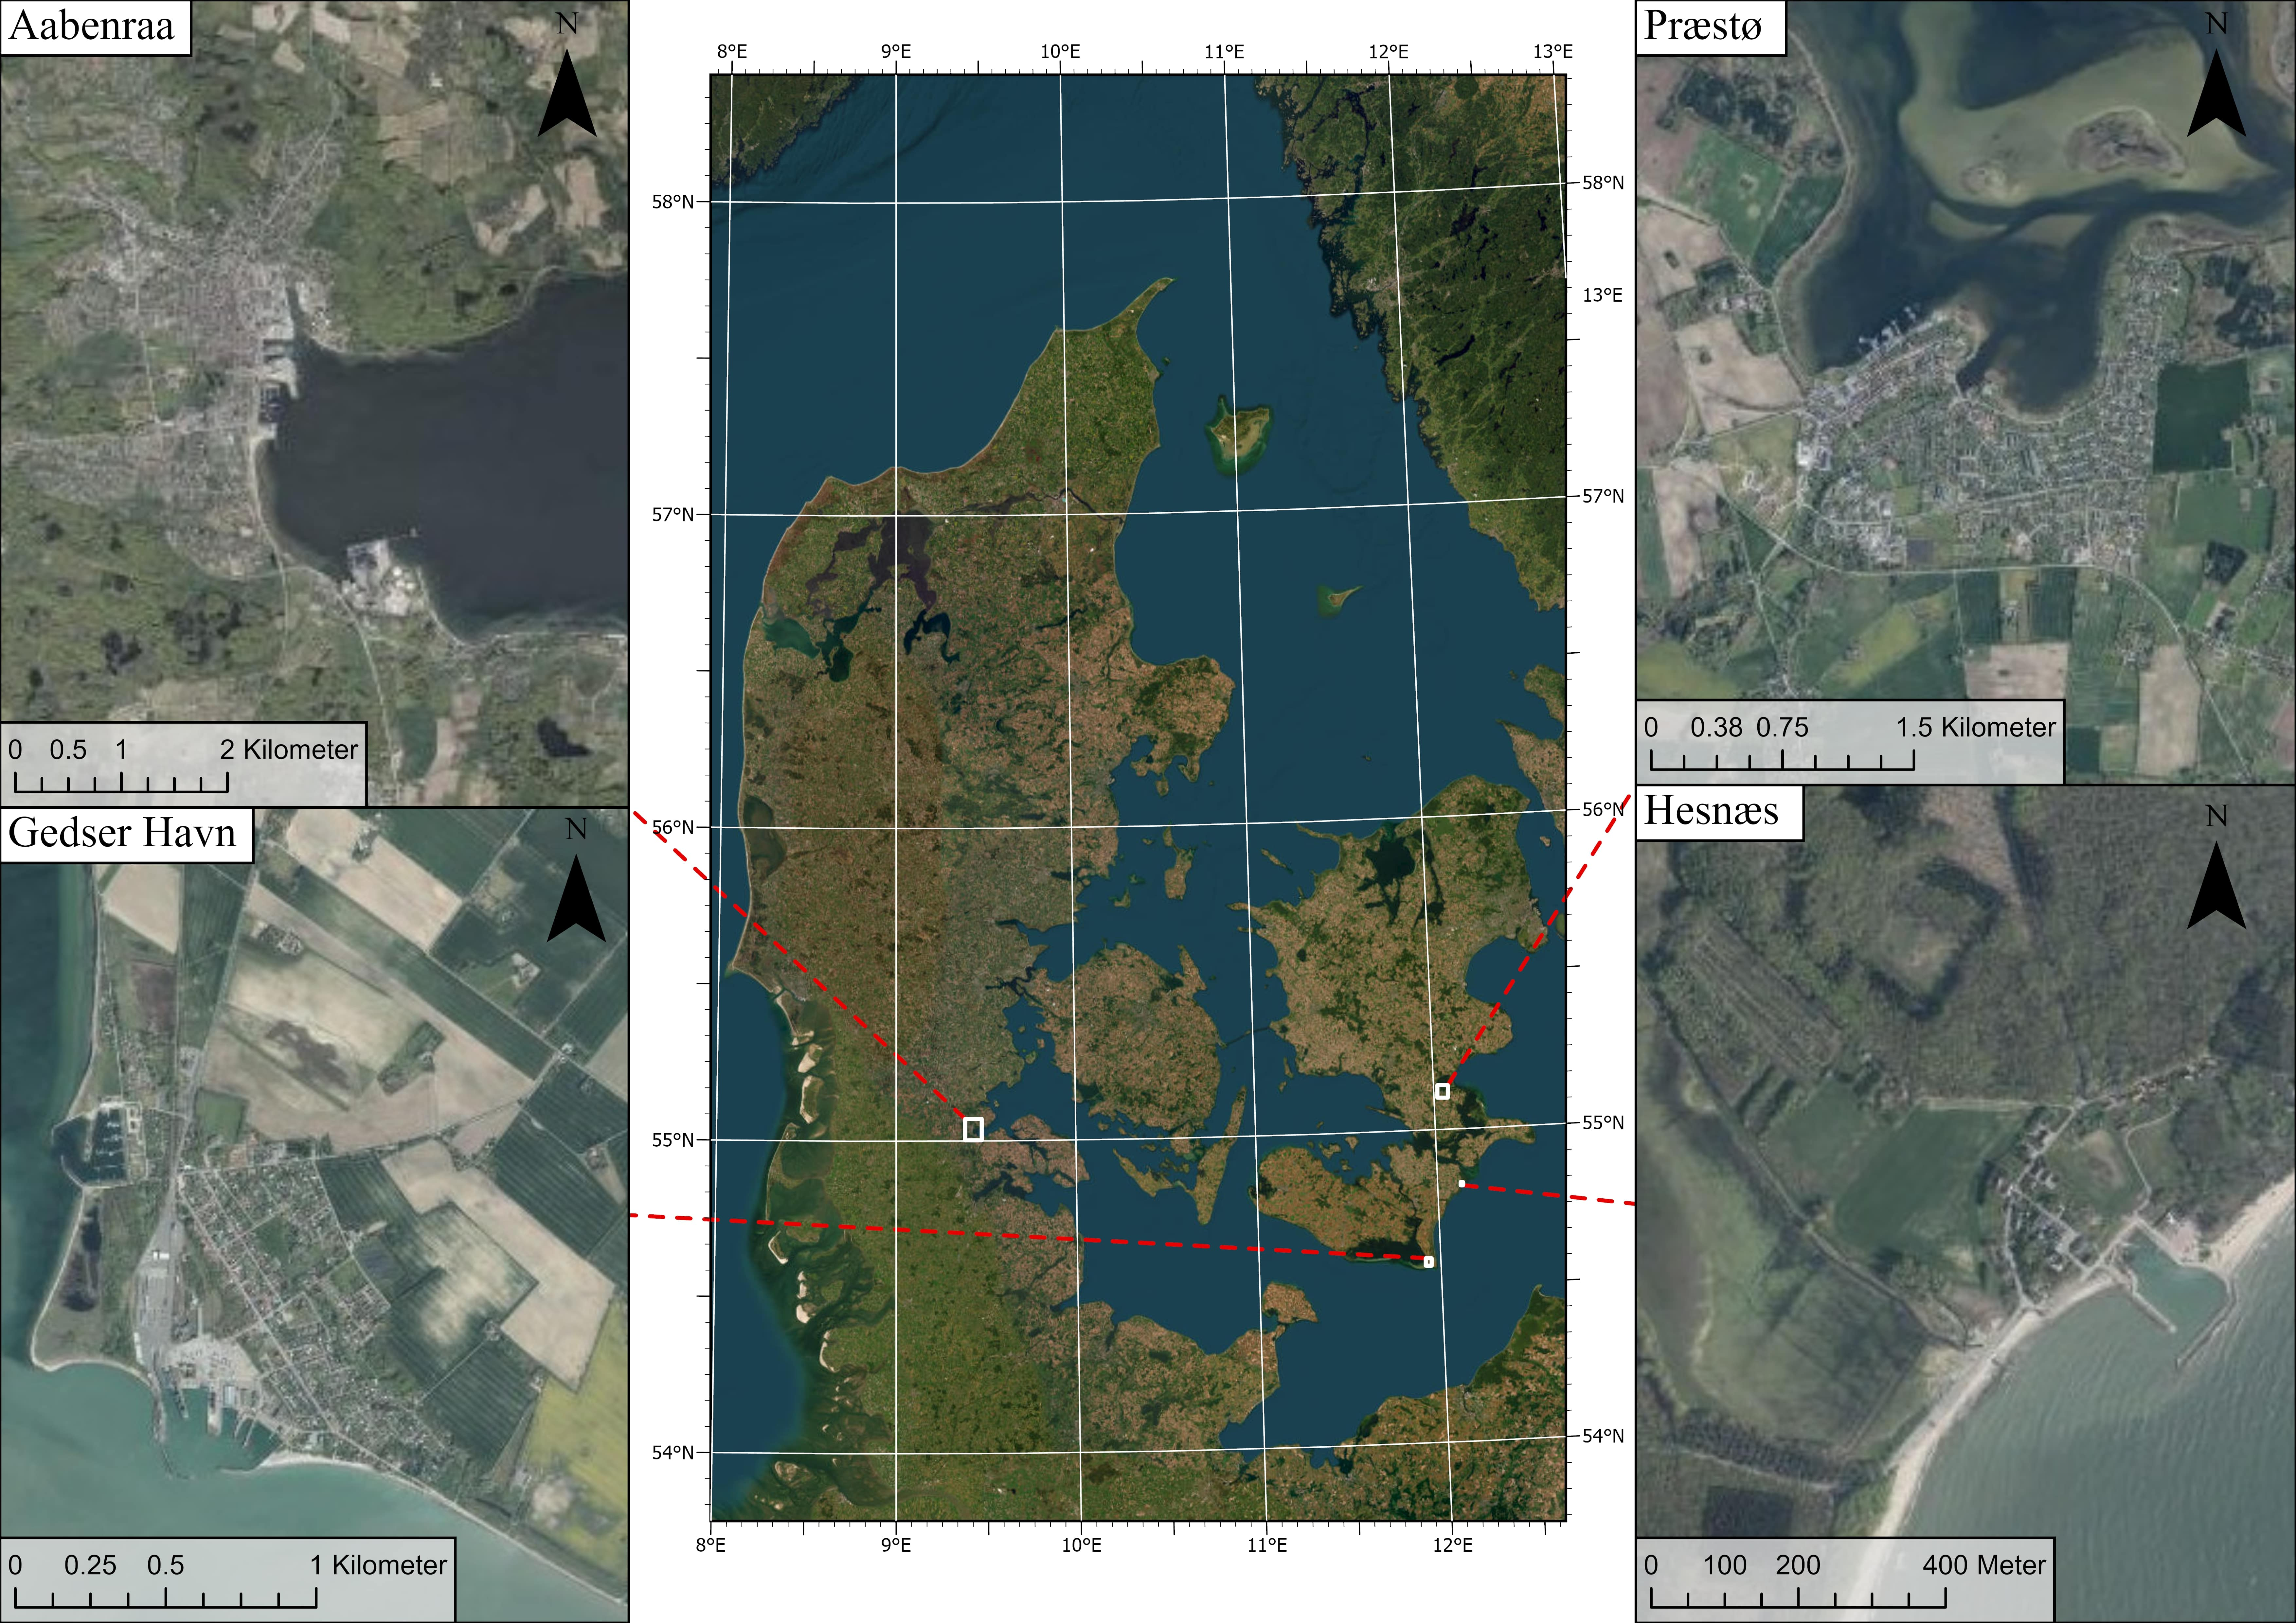
\includegraphics[width=1\linewidth]{images/studieområder/oversigtskort.jpg}
    \caption{Oversigtskort over studieområderne: Aabenraa, Gedser Havn, Hesnæs og Præstø. Baggrundskort fra ESRI og Klimadatastyrelsen}
    \label{Figur: Oversigtskort}
\end{figure}

Aabenraa er en by i det sydøstlige Sønderjylland. Byen er beliggende i Aabenraa kommune for enden af den ca. 10 km lange Aabenraa fjord. Byen har en befolkning på 16500 og er den niende største by i Region Syddanmark \citep{danmarks_statistisk_mobile_nodate}. Byen består af to store industri havne, Aabenraa og Ensted, og er en vigtigt for skibstrafik med 380 anløbte skibe i 2022 \citep{aabenraa_havn_aabenraa-havn-talogfakta2022_2022}.\\
Aabenraa oplevede den højeste officielle måling af vandstand under stormfloden den 20.-21. oktober 2023 på 2,16 meter over DVR90 (figur \ref{Subfig: Aabenraa vandstand}). \\

Gedser Havn er en by på sydspidsen af Falster i Guldborgsund kommune. Gedser Havn fungerer som en aktiv fiskeri havn og som en færgehavn til den tyske havn Warnemünde ved Rostock. Byen har haft en indbyggertal på 670 i 2024 \citep{danmarks_statistisk_mobile_nodate} og er Danmarks sydligste by. \\
Under stormfloden den 20 oktober 2023 oplevede Gedser Havn en vandstandsstigning på 1,89 meter over DVR90 (figur \ref{Subfig: Gedser vandstand}), den højeste vandstand siden 1892, og stoppede for færgetrafikken til Tyskland frem til formiddagen den 21. oktober \citep{tiirikainen_sadan_2023}.\\
\begin{figure}[H]
    \begin{subfigure}[b]{0.5\textwidth}
        \centering
        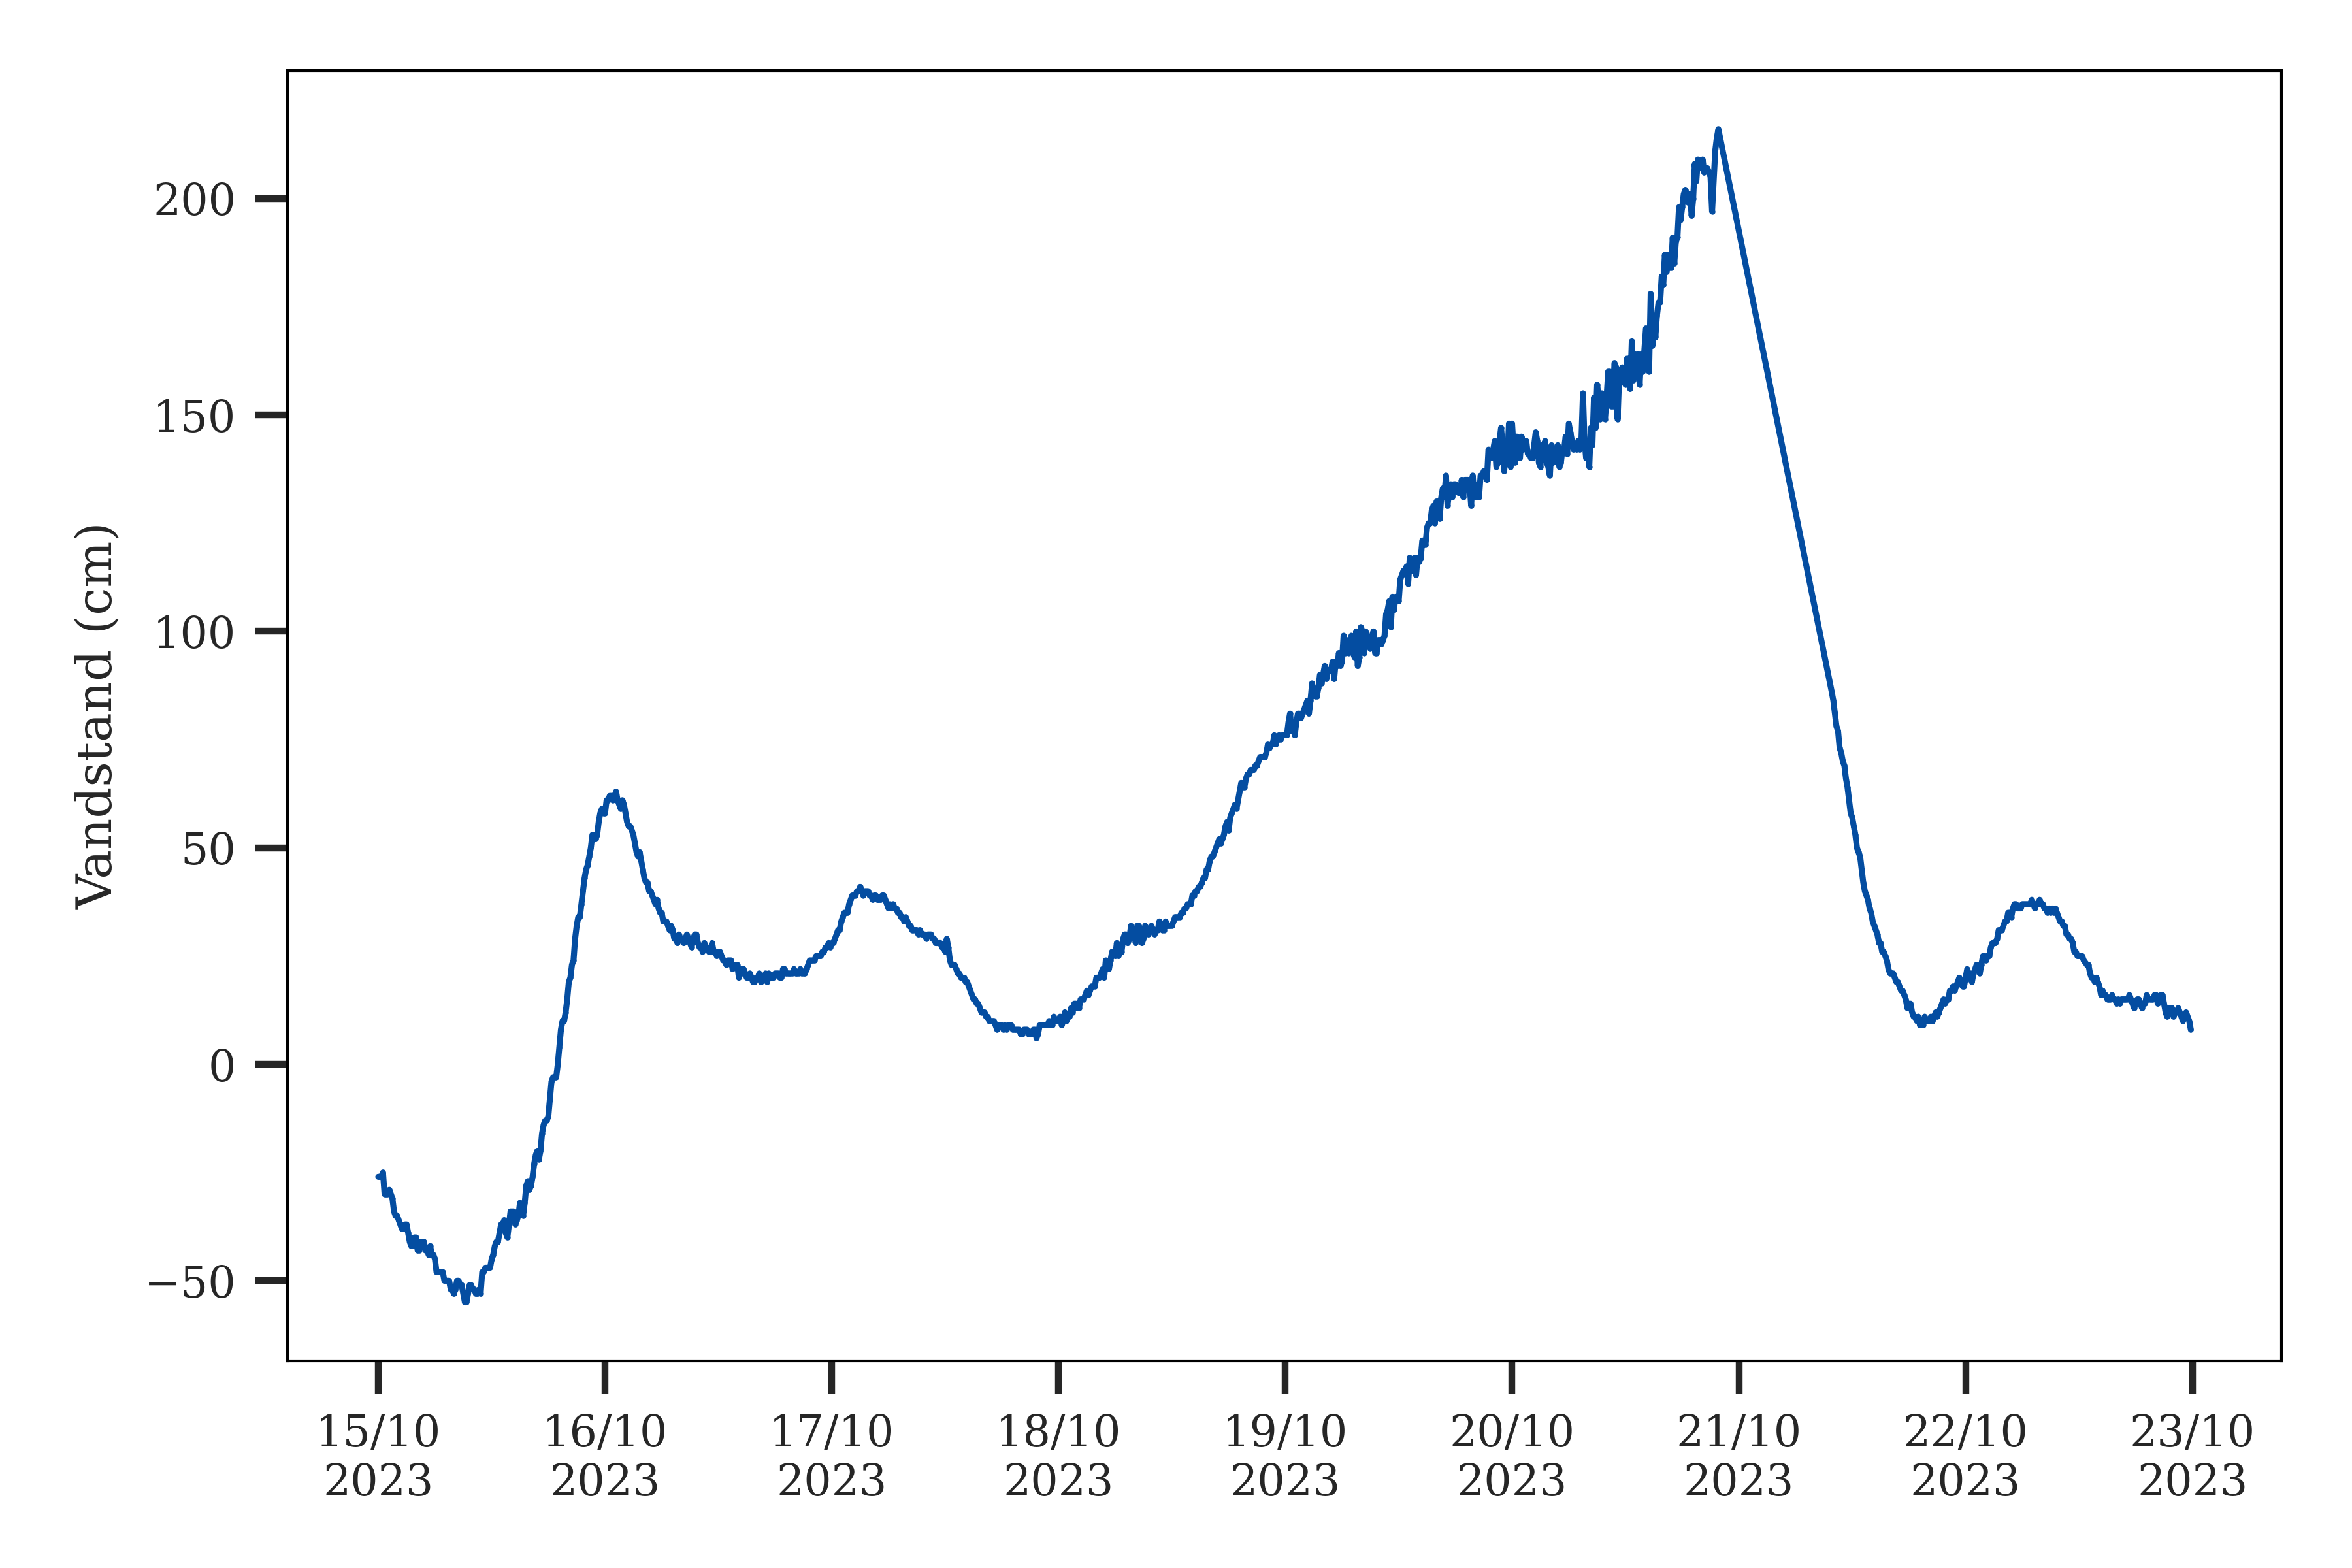
\includegraphics[width=1\textwidth]{images/vandstands_grafer/vandstand_aabenraa_vandstandsplot.png}
        \caption{Vandstanden i Aabenraa fra 15. til 23. oktober 2023.}
        \label{Subfig: Aabenraa vandstand}
    \end{subfigure}
    \hspace{0.2cm}
    \begin{subfigure}[b]{0.5\textwidth}
        \centering
        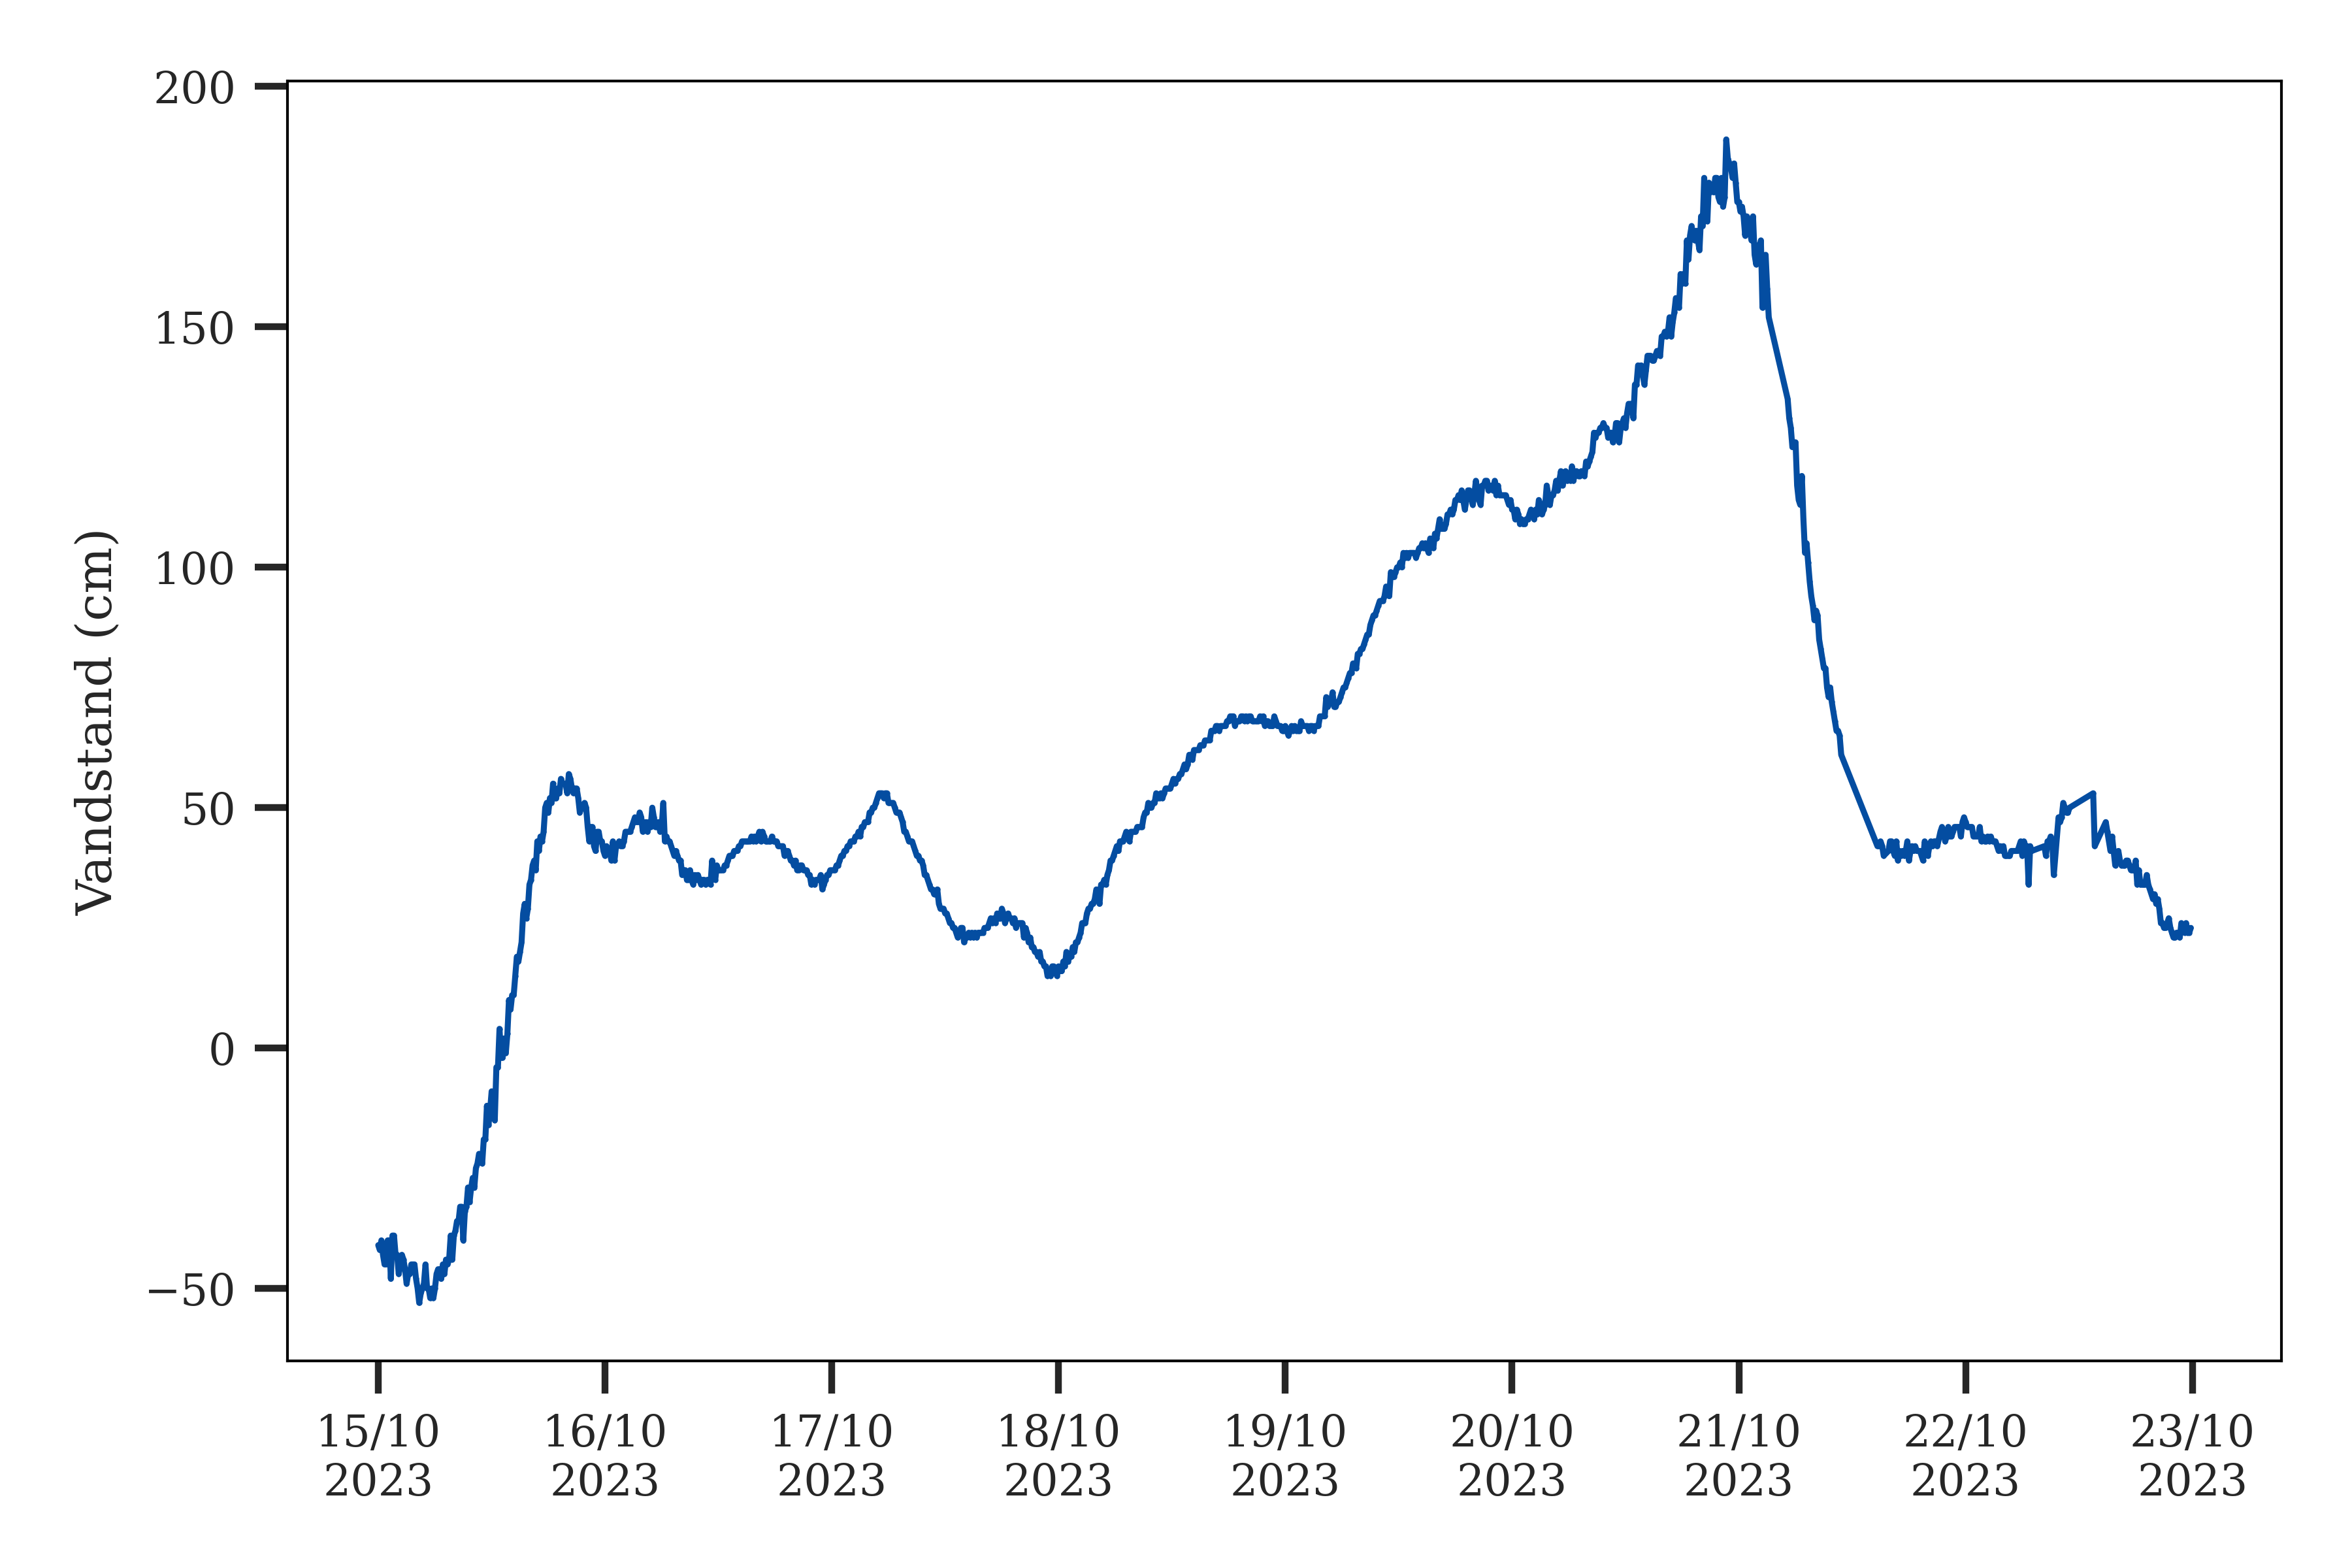
\includegraphics[width=1\textwidth]{images/vandstands_grafer/vandstand_gedser_vandstandsplot.png}
        \caption{Vandstanden i Gedser Havn fra 15. til 23. oktober 2023}
        \label{Subfig: Gedser vandstand}
    \end{subfigure}
    \vspace{0.2cm}
    \begin{subfigure}[b]{0.5\textwidth}
        \centering
        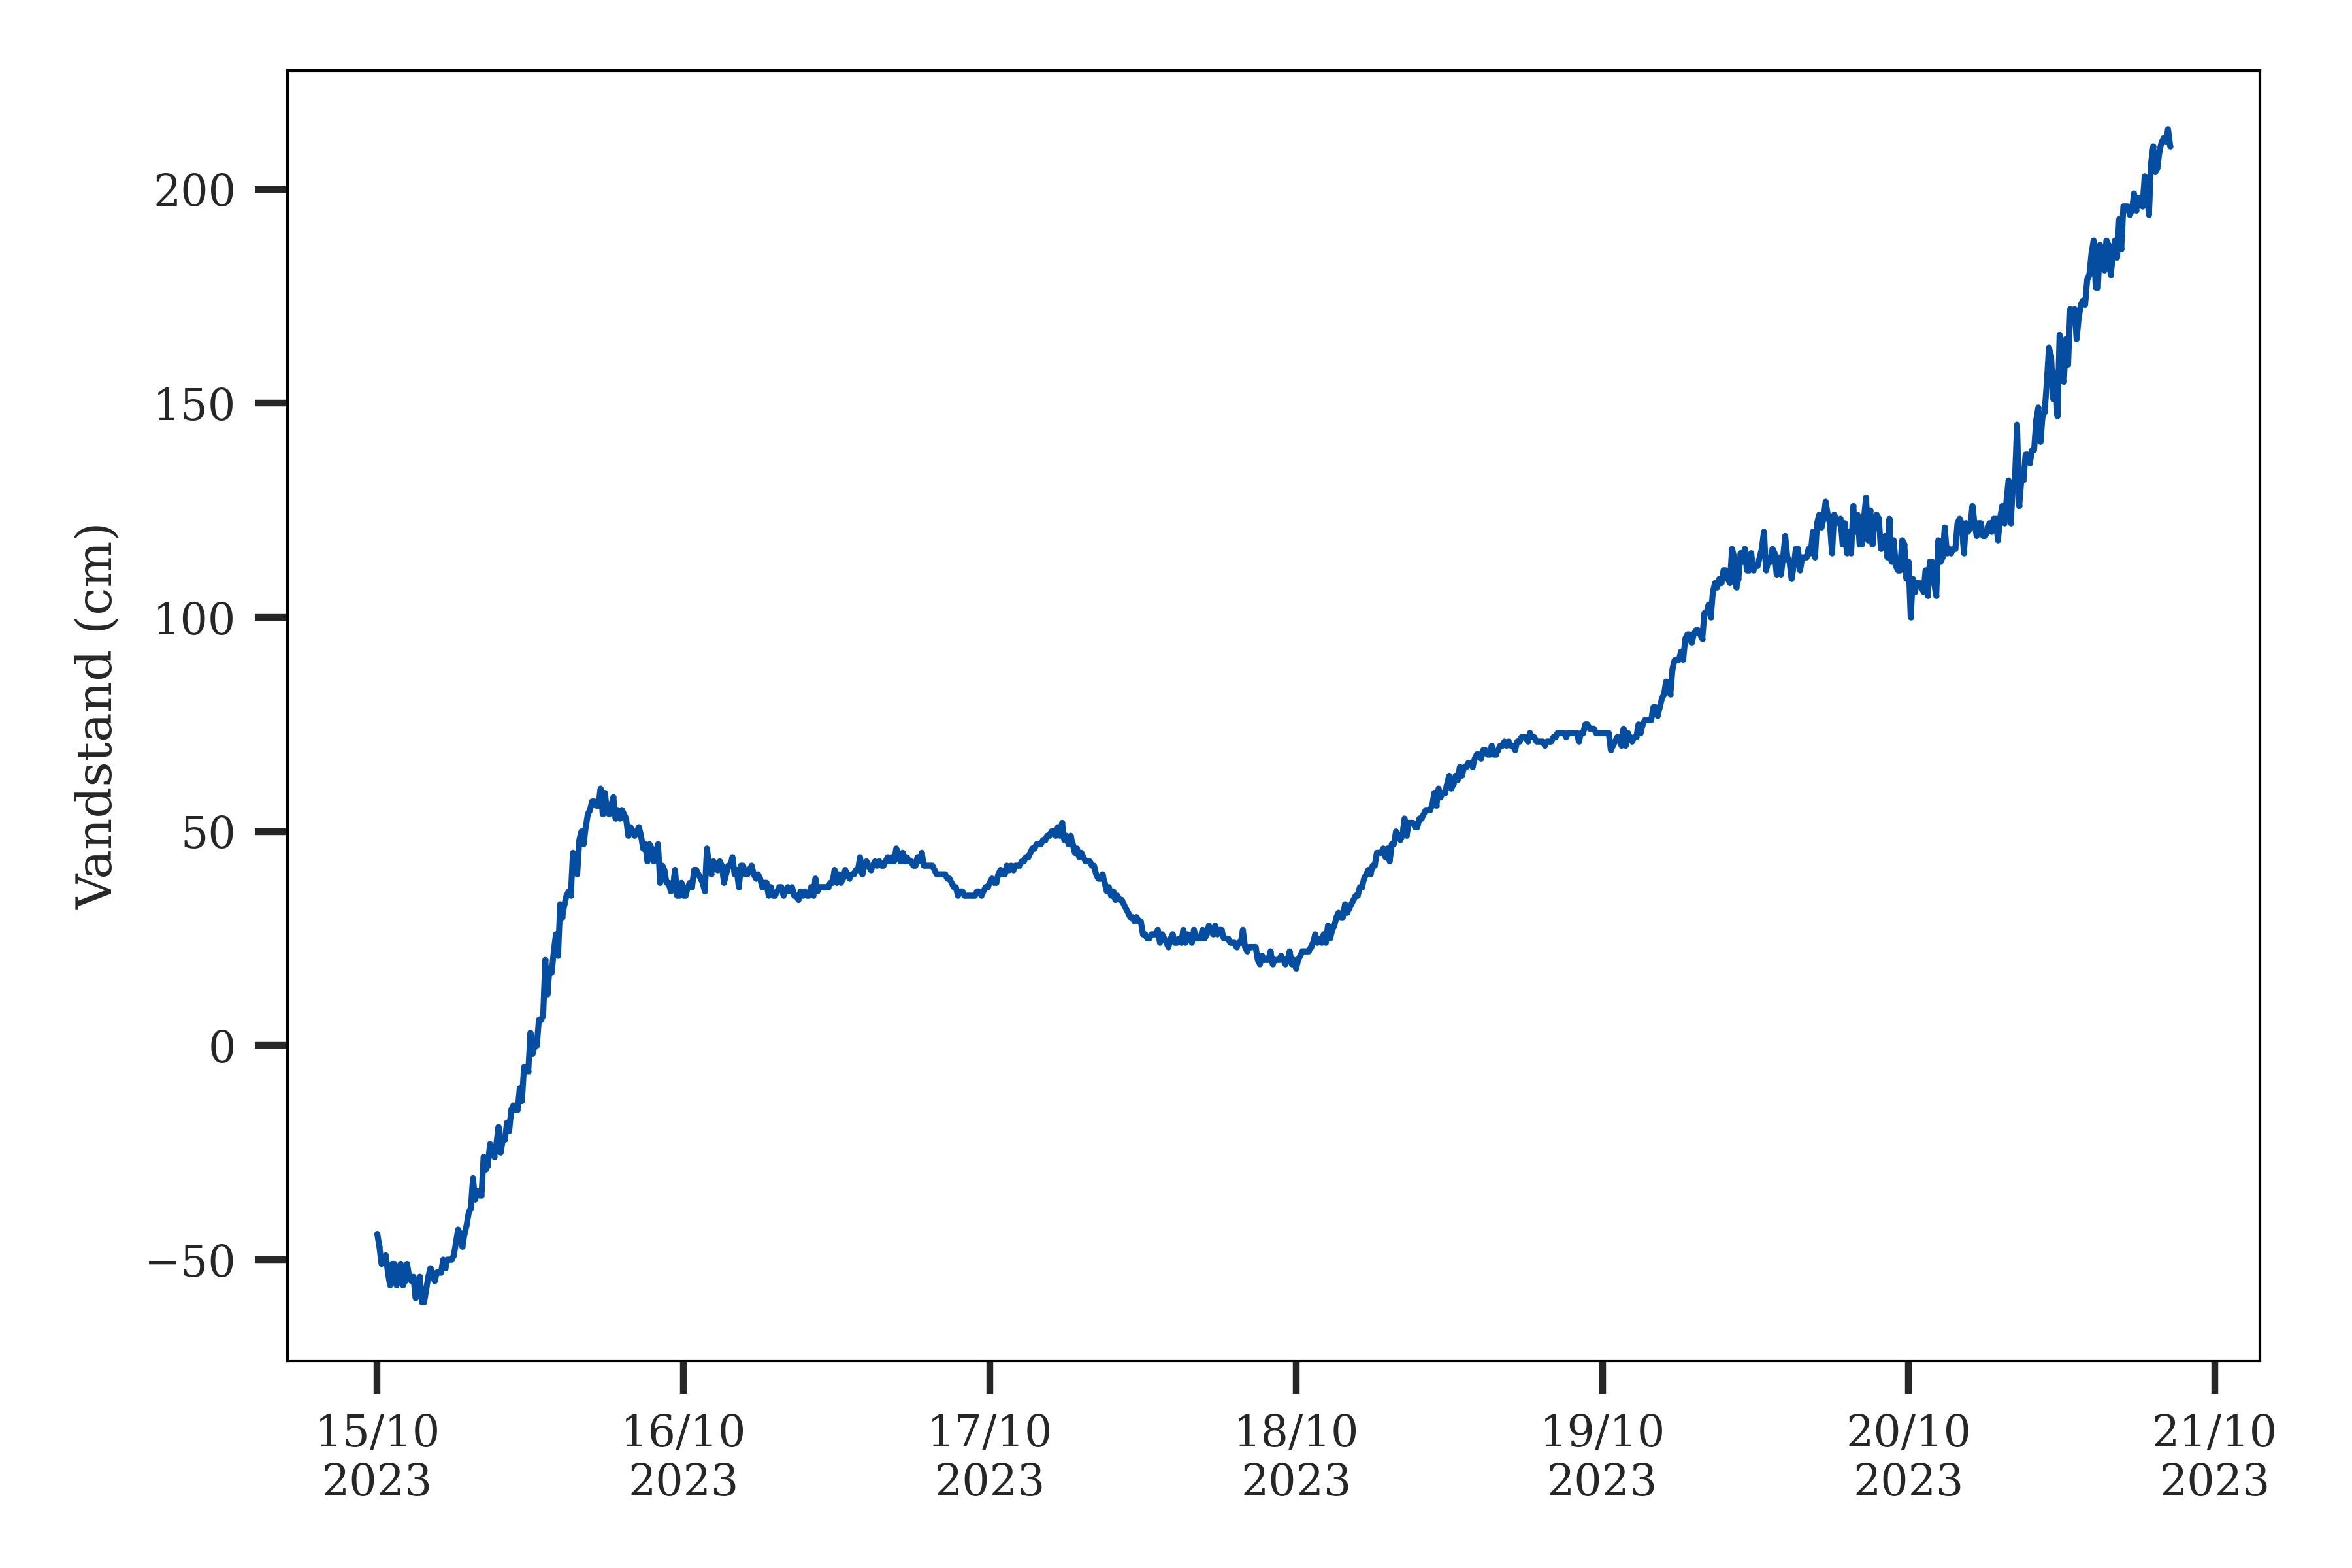
\includegraphics[width=1\textwidth]{images/vandstands_grafer/vandstand_hesnaes_vandstandsplot.png}
        \caption{Vandstanden i Hesnæs fra 15. til 21. oktober 2023}
        \label{Subfig: Hesnæs vandstand}
    \end{subfigure}
    \hspace{0.2cm}
    \begin{subfigure}[b]{0.5\textwidth}
        \centering
        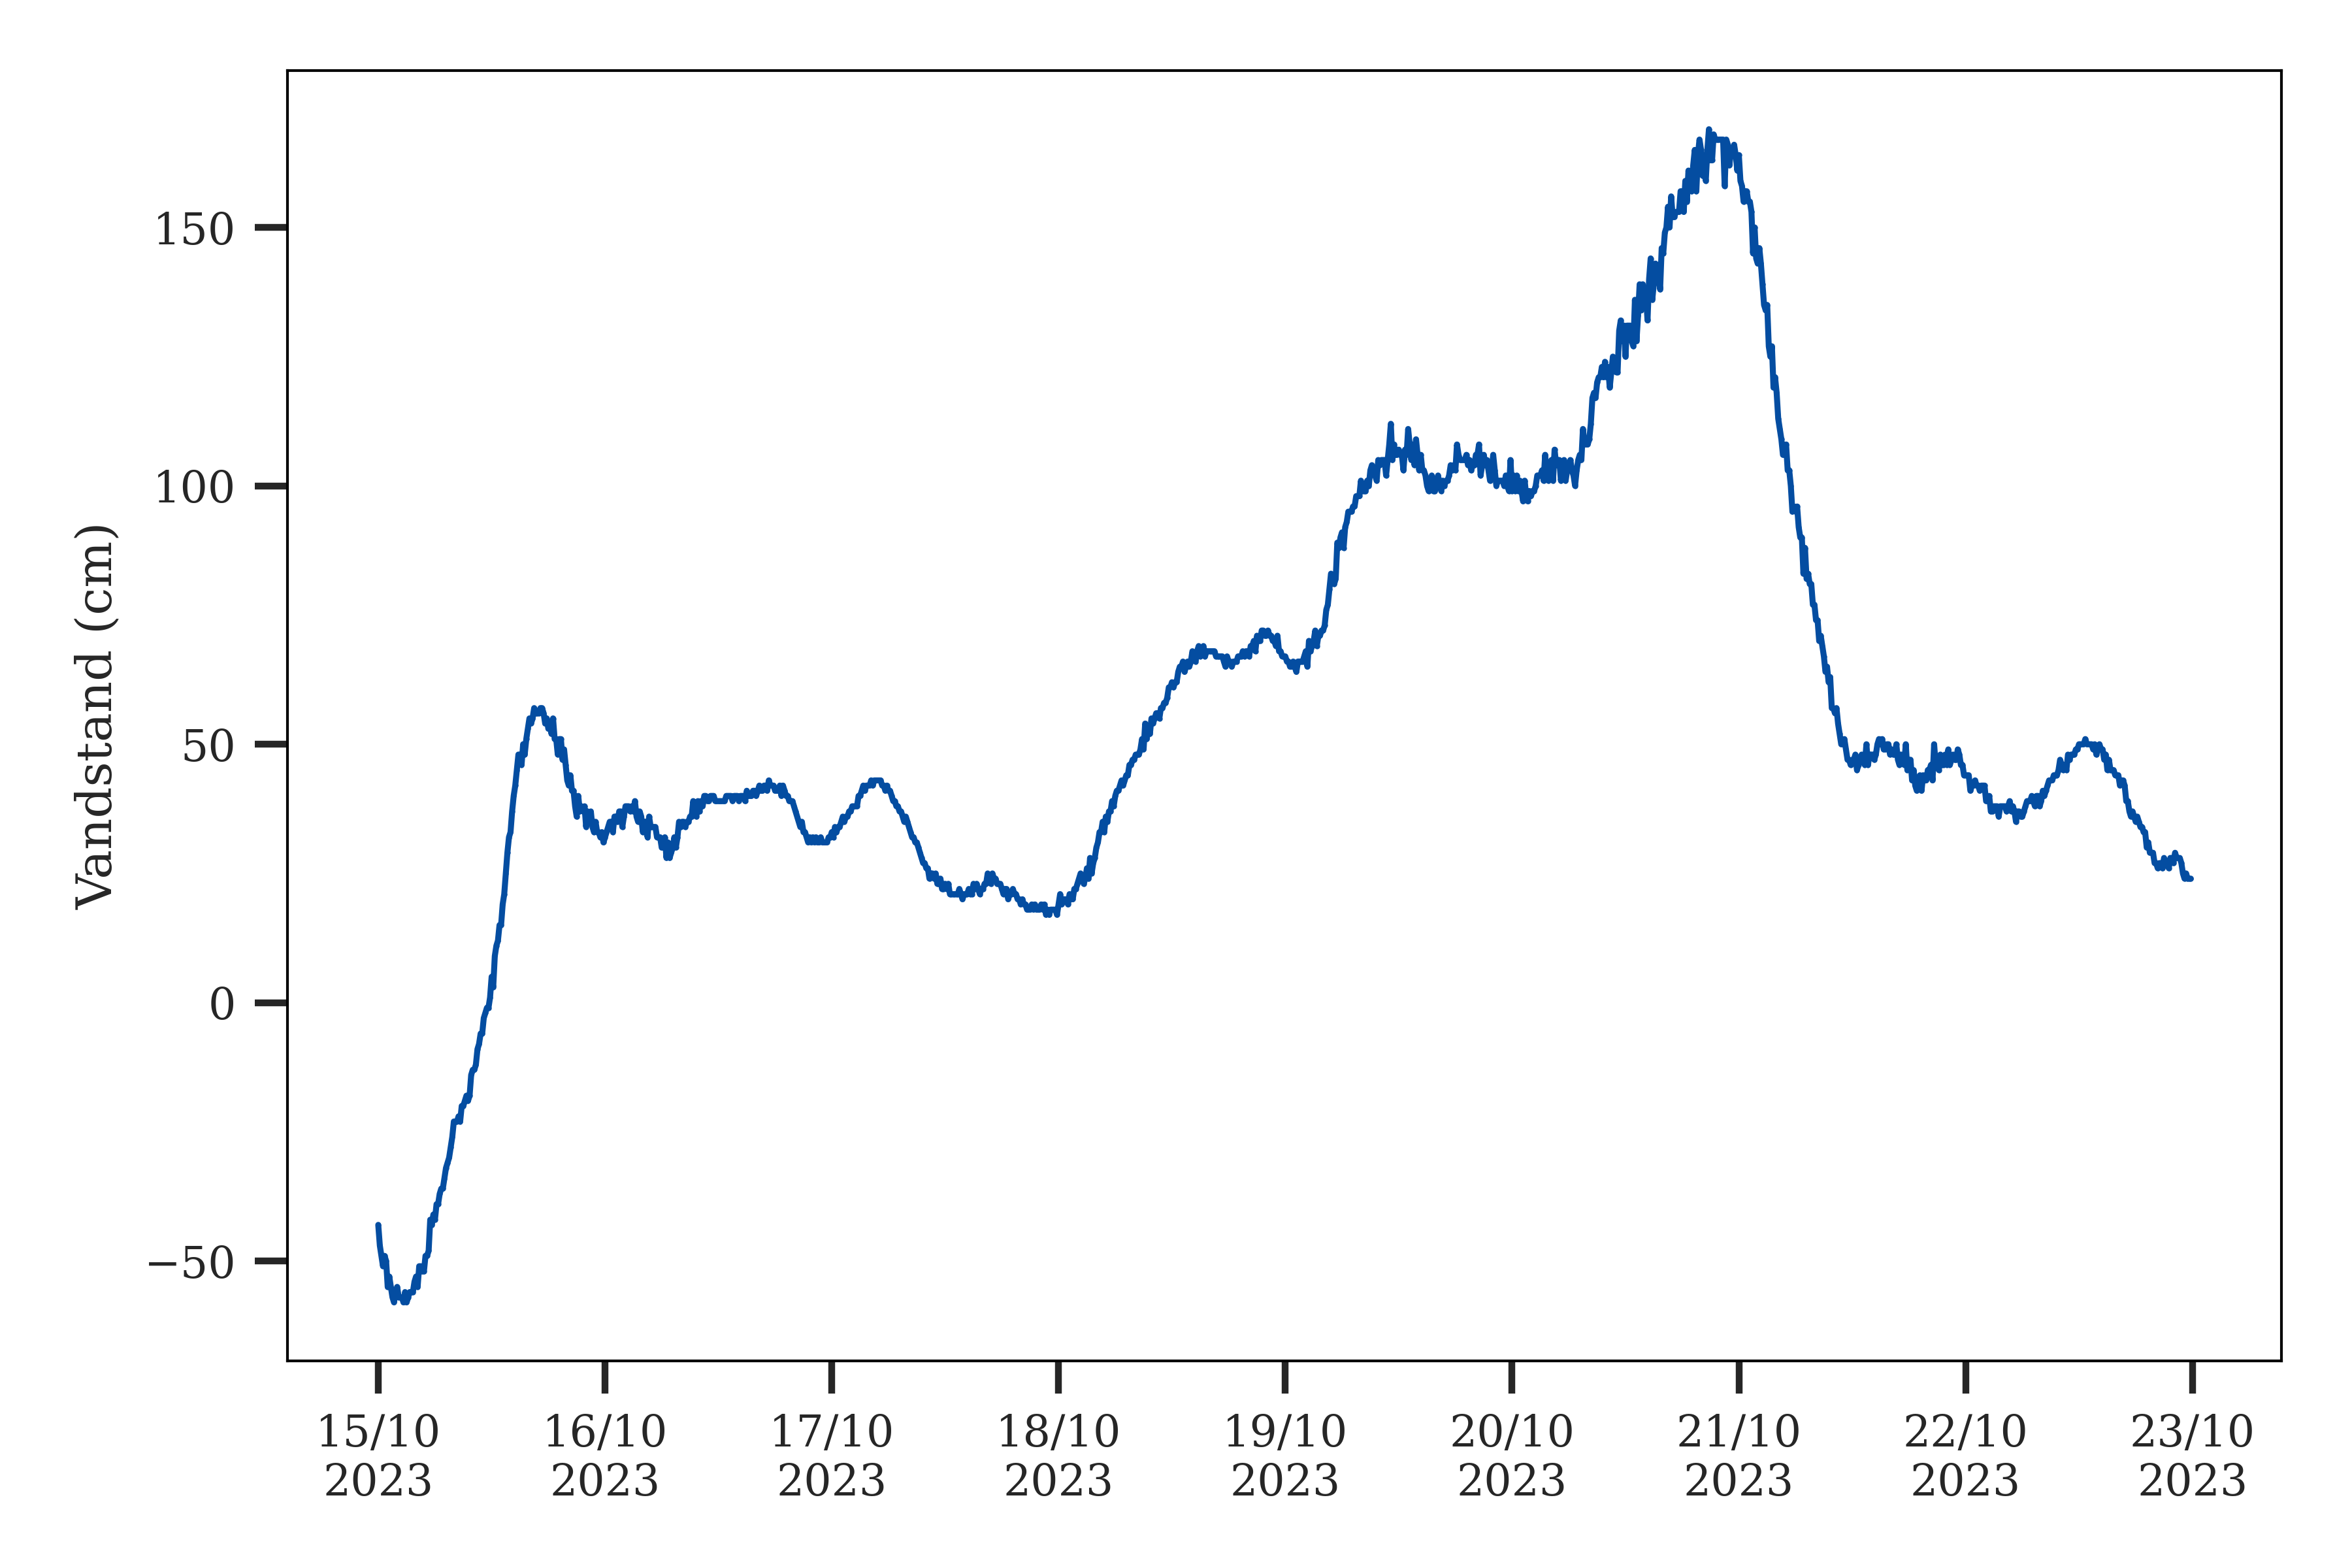
\includegraphics[width=1\textwidth]{images/vandstands_grafer/vandstand_praestoe_roedvig_vandstandsplot.png}
        \caption{Vandstanden i Rødvig fra 15. til 23. oktober 2023}
        \label{Subfig: Rødvig vandstand}
    \end{subfigure}
    \caption{Vandstanden i studieområderne Aabenraa, Gedser Havn, Hesnæs og Rødvig fra den 15. til 23. oktober. Kilde: Data stammer fra DMI og DMI Frie Data API-resource}
    \label{Figur: Vandstandsdata}
\end{figure}
Hesnæs er et lille fiskerleje og landsby på det østlige Falster i Guldborgsund kommune. Hesnæs fungerer som en havn og er den eneste på Falsters østkyst. Hesnæs er beliggende inde mellem to skove: Corselitze skov mod nord og Bønnet skov mod syd, som begge går helt ud til skrånede klinter ud til Østersøen. \\
Hesnæs blev særdeles hårdt ramt af stormfloden den 20 oktober 2023, hvor der blev officielt målt 2,10 m vandstand over DVR90. Uofficielle målinger nåede helt op på 2,39 meter over DVR90, men måleren gik i stykker kort tid efter (figur \ref{Subfig: Hesnæs vandstand}). Meget af Hesnæs havn blev svært beskadet af stormen, især den ydre mole af havnen blev ødelagt og lystbådhavnen blev dermed sat ud af drift på ubestemt tid. \\

Præstø er en havneby og en tidligere købstad i Vordingborg Kommune på Sjælland. Byen er beliggende i den sydlige del af Præstø Fjord, bag halvøen Feddet i bunden af Faxe Bugt. Tværs igennem byen løber tunneldalen Tubæk Å, et vandløb der deler byen mellem et nordligt handelscentrum og et sydligt boligkvarter. Byen har en befolkningstal på 3939 i 2025 \citep{danmarks_statistisk_mobile_nodate} og er kommunens anden største by. \\
Under stormfloden den 20 oktober 2023 blev store dele af Præstøs handelscentrum oversvømmet, især efter sluseporten der bruges til tilbageholde vandet i Tubæk Å, brød sammen \citep{uldall_sluseport_2023}. Der er ingen officielle målinger om vandstandshøjden i Præstø under stormfloden, da den nærmeste målestation er placeret længere opstrøms af Tubæk Å. \cite{cowi_praesto_2025} giver et skøn på at vandstanden var ca. 40 cm højere end i Rødvig Havn i Stevs Kommune ca. 25 km nordøst fra Præstø. Dette giver en vandstand på 2 meter over DVR90 under stormfloden i Præstø (figur \ref{Subfig: Rødvig vandstand}).

